\section{La corbeille}
La corbeille est un dernier lieu de stockage des donn�es effac�es par
les enseignants et m�me l'administrateur. Cette zone, seulement
accessible par l'administrateur de l'application, permet soit une
suppression d�finitive des donn�es soit une restauration.\\
De plus, pour faciliter sa consultation, la corbeille permet plusieurs
affichages. 

\begin{flushleft}
\scalebox{0.5}{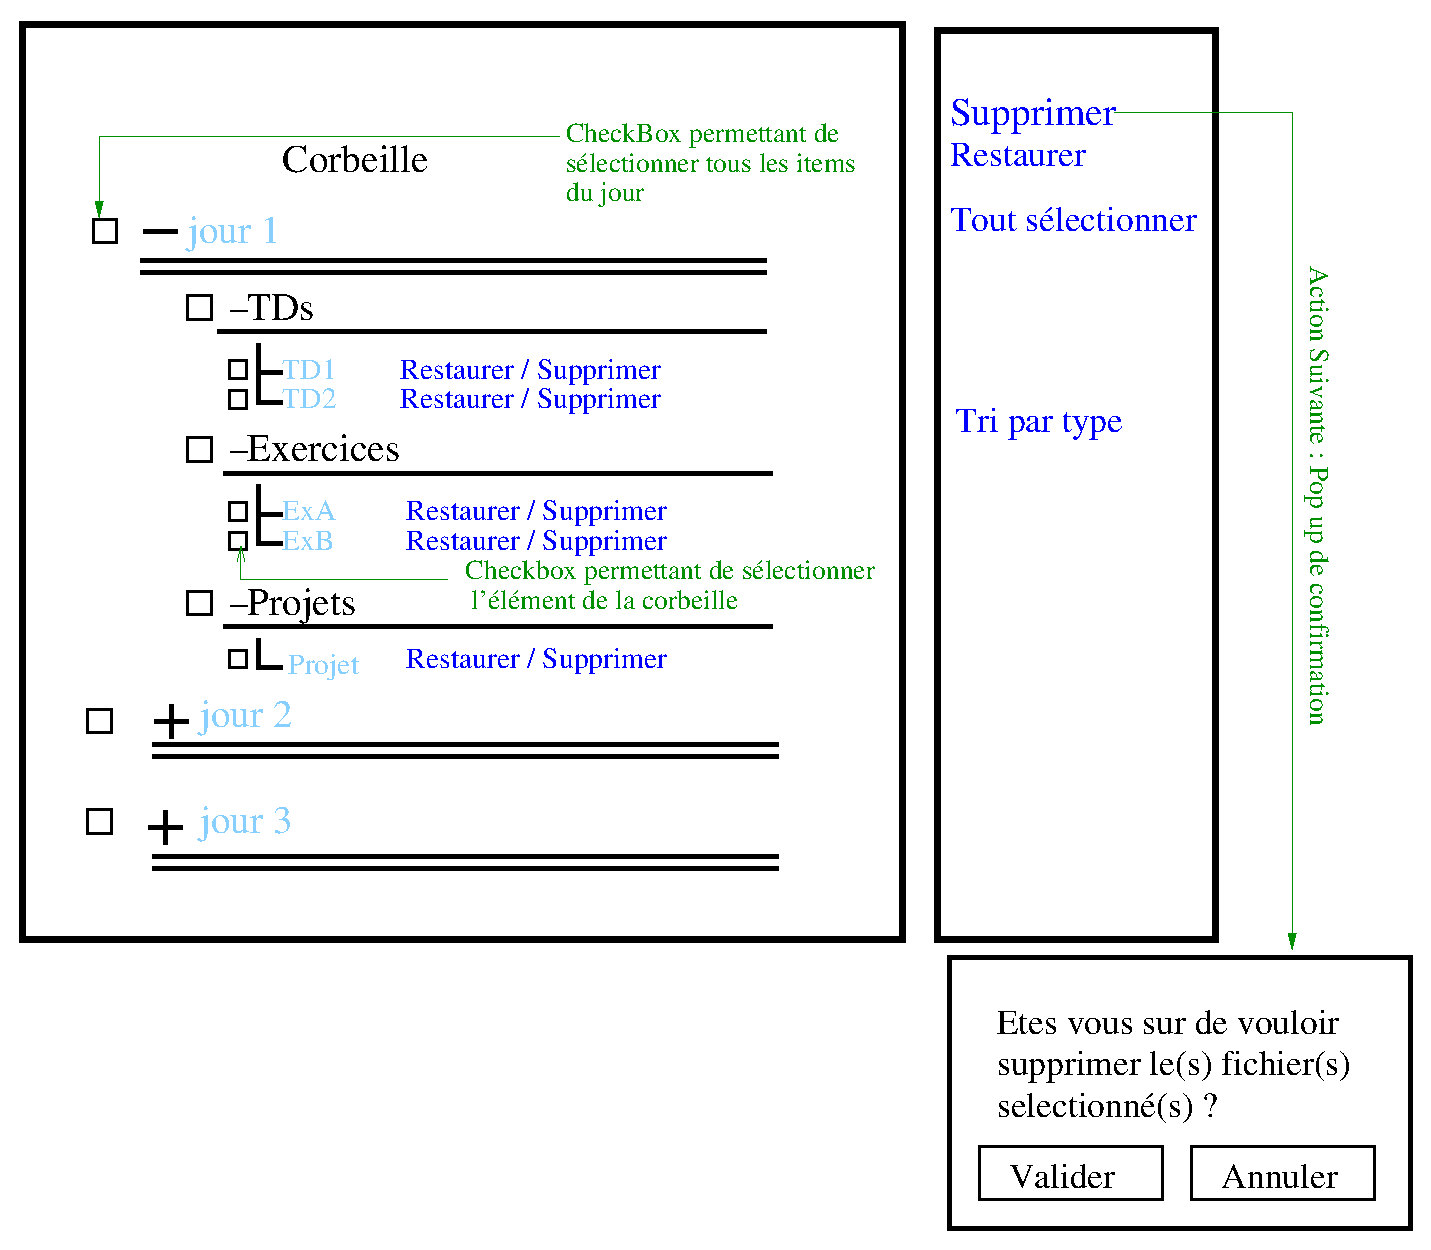
\includegraphics{../eps/corbeilleTriDate.eps}}\\
{\it Corbeille tri� par date}
\end{flushleft}

\begin{flushleft}
\scalebox{0.5}{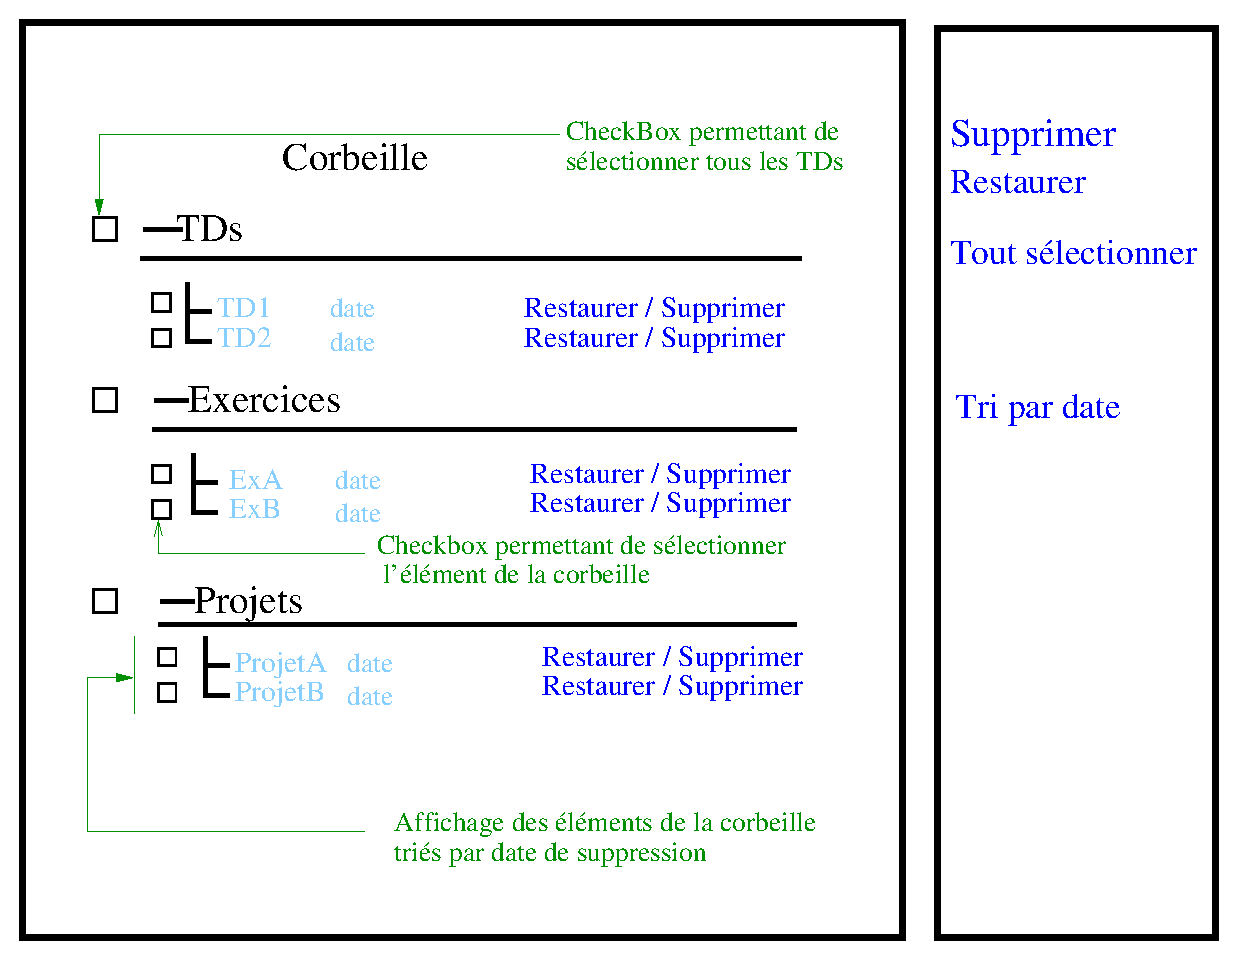
\includegraphics{../eps/corbeilleTriType.eps}}\\
{\it Corbeille tri� par type}
\end{flushleft}


La corbeille permet de restaurer les donn�es s�lectionn�es par
l'administrateur. L'application offre la possibilit� de s�lectionner
certains �lements ou un groupe d'�l�ments. 
\begin{flushleft}
\scalebox{0.5}{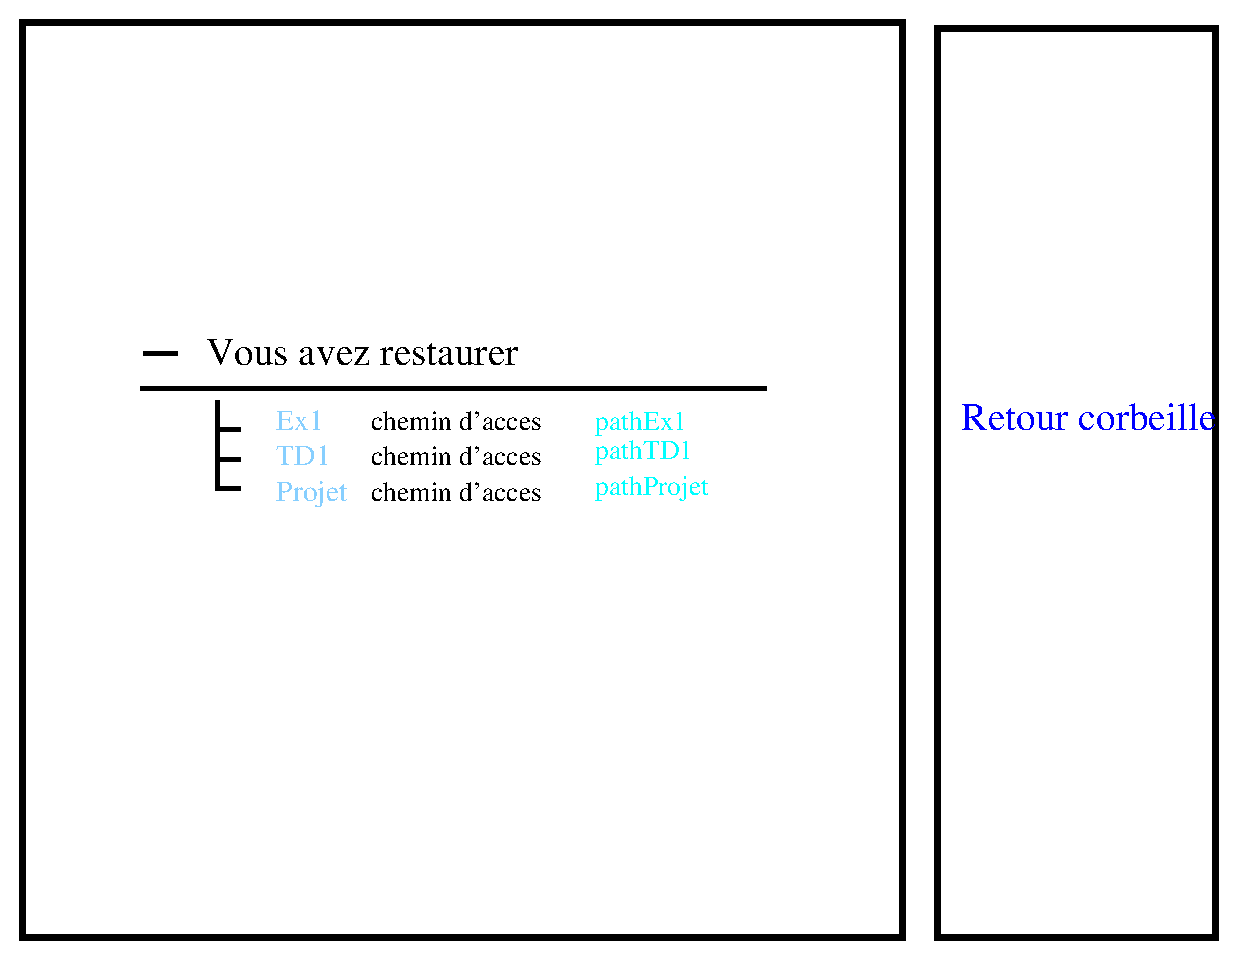
\includegraphics{../eps/corbeilleListRestaur.eps}}\\
{\it Corbeille apr�s restauration}
\end{flushleft}


